%% BEAMER THEME FLIP 2012: Main tex file for compiling
%$ Compile this file.
%%
%% Copyright 2012 by Flip Tanedo
%% This file may be distributed and/or modified
%% 	1. under the LaTeX Project Public License and/or
%% 	2. under the GNU Public License.
%%
%% If you e-mail Flip (pt267@cornell.edu) to say that you
%% like this style file, then it would make him smile.

%% Please see notes.txt for comments on Beamer Theme Flip 2013
%% By default, this template is meant to be run with XeLaTeX (for fonts)
%% To run in PDFLaTeX, remove fontspec and any font commands

%% Discussion of Beamer vs XeLaTeX vs LuaLaTeX
%% http://tex.stackexchange.com/questions/29497/xelatex-preventing-beamer-from-using-different-backgrounds



\documentclass[12 pt]{beamer}
\usetheme[
	bullet=circle,		% Other option: square
	bigpagenumber,		% circled page number on lower right
	topline=true,			% colored bar at the top of the frame
	shadow=false,			% Shading for beamer blocks
	watermark=BG_lower,	% png file for the watermark
	]{Flip}


\newcommand{\titleimage}{title}			% Custom title
\newcommand{\tanedo}{tanedolight}		% Custom author name
\newcommand{\CMSSMDM}{CMSSMDMlight.png}	% light background plot


%%%%%%%%%%
% FONTS %
%%%%%%%%%%

%% Default font: lmodern, doesn't require fontspec % solves some default warnings
\usepackage[T1]{fontenc}
\usepackage{lmodern}
%\usepackage{sfmath}		% Sans Serif Math, off by default

%% Protects fonts from Beamer screwing with them
%% http://tex.stackexchange.com/questions/10488/force-computer-modern-in-math-mode
\usefonttheme{professionalfonts}


%% XeLaTeX fonts: (comment out if you don't use XeLaTeX)

%% For advanced fonts: access local OS X fonts
\usepackage[no-math]{fontspec}
%% This template uses typical OS X and Adobe fonts
\defaultfontfeatures{Mapping=tex-text}	% This seems to be important for mapping glyphs properly

\setmainfont{PT Sans}			% Beamer ignores "main font" in favor of sans font
\setsansfont{PT Sans}			% This is the font that beamer will use by default
% \setmainfont{Gill Sans Light}		% Prettier, but harder to read

\setbeamerfont{title}{family=\fontspec{PT Sans}}


% \newcommand{\handwriting}{\fontspec{augie}} % From Emerald City, free font
\newcommand{\handwriting}{}	% If you prefer no special handwriting font or don't have augie

%% Gill Sans doesn't look very nice when boldfaced
%% This is a hack to use Helvetica instead
%% Usage: \textbf{\forbold some stuff}
\newcommand{\forbold}{\fontspec{PT Sans}}
% \newcommand{\forbold}{} % if you want no special boldface



%%%%%%%%%%%%%%%%%%%%%%%%
% Usual LaTeX Packages %
%%%%%%%%%%%%%%%%%%%%%%%%

\usepackage{xargs}
\usepackage{amsmath}
\usepackage{amsfonts}
\usepackage{amssymb}
\usepackage{graphicx}
\usepackage{mathrsfs} 			% For Weinberg-esque letters
\usepackage{cancel}				% For "SUSY-breaking" symbol
\usepackage{slashed}            % for slashed characters in math mode
\usepackage{bbm}                % for \mathbbm{1} (unit matrix)
\usepackage{amsthm}				% For theorem environment
\usepackage{multirow}			% For multi row cells in table
\usepackage{arydshln} 			% For dashed lines in arrays and tables
\usepackage{tikzfeynman}		% For Feynman diagrams
% Syntax Highlighting in LaTeX, need pygments
% Must build with xelatex -shell-escape -enable-8bit-chars.
\usepackage{algorithm,algpseudocode}
\usepackage{tikz}
\usepackage{minted}
\usepackage{braket} % needed for \Set
% textblock
%\usepackage{textpos}
% Typesetting theorems (AMS style)
\usepackage{amsthm}
% ifthenelse
\usepackage{ifthen}
% math equations
\usepackage{bm}

% \usepackage{subfig}           % for sub figures
% \usepackage{young}			% For Young Tableaux
% \usepackage{xspace}			% For spacing after commands
% \usepackage{wrapfig}			% for Text wrap around figures
% \usepackage{framed}


\graphicspath{{images/}}	% Put all images in this directory. Avoids clutter.


\usetikzlibrary{backgrounds}
\usetikzlibrary{mindmap,trees}	% For mind map
% http://www.texample.net/tikz/examples/computer-science-mindmap/

% DCMMC: for university logo
\newif\ifplacelogo % create a new conditional
\placelogotrue % set it to true

% SOME COMMANDS THAT I FIND HANDY
% \renewcommand{\tilde}{\widetilde} % dinky tildes look silly, dosn't work with fontspec
\newcommand{\comment}[1]{\textcolor{comment}{\footnotesize{#1}\normalsize}} % comment mild
% DCMMC: Command already defined!
\renewcommand{\Comment}[1]{\textcolor{Comment}{\footnotesize{#1}\normalsize}} % comment bold
\newcommand{\COMMENT}[1]{\textcolor{COMMENT}{\footnotesize{#1}\normalsize}} % comment crazy bold
\newcommand{\Alert}[1]{\textcolor{Alert}{#1}} % louder alert
\newcommand{\ALERT}[1]{\textcolor{ALERT}{#1}} % loudest alert
%% "\alert" is already a beamer pre-defined


% DCMMC: 显示在页脚的作者,标题, 单位
\author[Wentao Xiao\quad {wentao.xiaoo@mail.dhu.edu.cn}]{Wentao Xiao}
\title[A demo for Flip's Beamer Theme]{A demo for Flip's Beamer Theme}
\institute{Donghua University}
% DCMMMC: 显示在首页的日期
\date{\today}

% color for minted
\definecolor{friendlybg}{HTML}{f0f0f0}

%The next block of commands puts the table of contents at the
%beginning of each section and highlights the current section:
\AtBeginSection[]
{
	% DCMMC: disable university logo for TOC
	\placelogofalse
	\begin{frame}
		\frametitle{Contents}
		\tableofcontents[currentsection]
	\end{frame}
	\placelogotrue
}

\begin{document}


%%%%%%%%%%%%%%%%%%%%%%%%
% Additional  settings %
%%%%%%%%%%%%%%%%%%%%%%%%

%% To use external nodes; http://www.texample.net/tikz/examples/beamer-arrows/
\tikzstyle{every picture}+=[remember picture]


%%%%%%%%%%%%%%%%%%%%%%%%
% Actual content below %
%%%%%%%%%%%%%%%%%%%%%%%%

%% It's much nicer to have all the content in a separate file
% DO NOT COMPILE THIS FILE DIRECTLY!
% This is included by the the driver file (FlipBeamerTemplate.tex).

{ %% This is a total kludge for a fancy title page background
%\setbeamertemplate{sidebar right}{\llap{
\includegraphics[width=\paperwidth,height=\paperheight]{BG_upper}}}
\setbeamertemplate{sidebar right}{\llap{
\includegraphics[height=\paperheight]{BG_DCMMC}}}
\begin{frame}[c]%{\phantom{title page}}
% The \phantom{title page} is a kludge to get the red bar on top
% \titlepage
\begin{center}
	% \includegraphics[width=7cm]{WarpedPenguinsReturn}

%	\begin{tikzpicture}%[show background grid] %% Use grid for positioning, then turn off
%		\node[inner sep=0pt,above right] (title)
%			{ \includegraphics[width=7cm]{\titleimage} };
%		% \node (title) at (1.5,1.5) {};
%	\end{tikzpicture}
	% A demo for Flip's Beamer Theme
	\vskip -3.5em
	\begin{flushright}
	\Large \textcolor[rgb]{0.1098,0.2706,0.5294}{{\fontspec{Noto Sans CJK SC} 面向语义分析的文本识别研究与实现}}
%	\quad
	\vskip 1.2em
	\large \textcolor[rgb]{0.1098,0.2706,0.5294}{{答辩人:肖文韬}
		{\fontspec{Comic Sans MS} 160800224}}

	\vskip .2em
	\large \textcolor[rgb]{0.1098,0.2706,0.5294}{指导老师:万燕}
	\end{flushright}
	% \includegraphics[width=7cm]{\titleimage}

	\vskip 2em
	% DCMMC: journal/conference and link
%	\footnotesize\textcolor{gray}{Journal of Cool Beans \texttt{[arXiv:1234.5678]}}
%	\vspace{.5em}

%	 \includegraphics[height=1.5cm]{\tanedo} \quad
%	{\fontspec{PT Sans} Wentao Xiao} \quad
%	\includegraphics[height=1.5cm]{CUasym}\\
%	\footnotesize\textcolor{gray}{Based on Flip Beamer Theme by Flip Tanedo @ Cornell University}\normalsize\\
	\textcolor{normal text.fg!50!Comment}{\textit{东华大学}, \today}
\end{center}
\end{frame}
}

%This block of code is for the table of contents after
%the title page
\placelogofalse
\begin{frame}
	\frametitle{目~~录}
	\tableofcontents
\end{frame}
\placelogotrue

\section{背景介绍}

\begin{frame}[c]{光学文本识别系统概览}
	\begin{columns}[t]
		\begin{column}[T]{7cm}
		\only<1>{
			光学文本识别(OCR):
			\begin{center}
				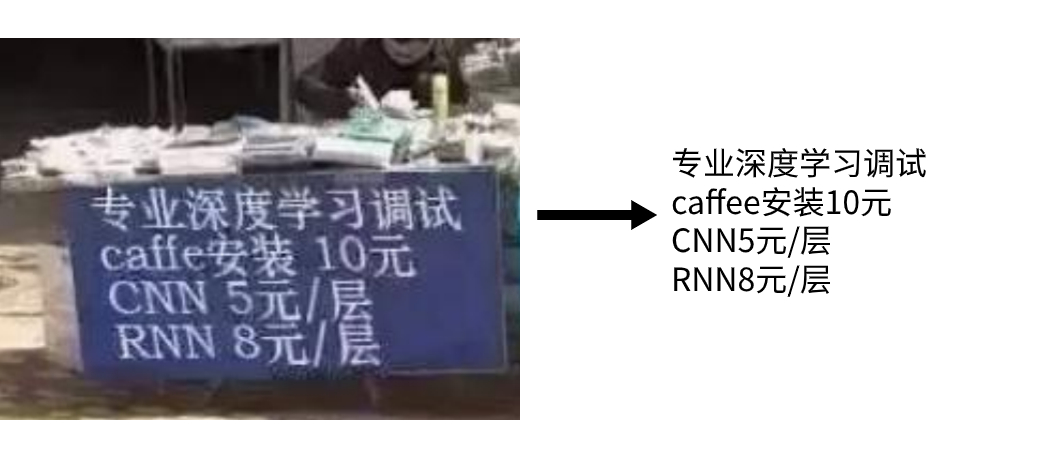
\includegraphics[width=\textwidth]{OCR_example.jpg}
			\end{center}
		}
		\only<2->{\ALERT{发现}:许多OCR任务的识别结果是一段\ALERT{自然语言},例如\Alert{“专业深度学习调试”} \\ \vspace{1.0em}}
		\only<3>{\ALERT{思考}:能否语义分析 OCR 识别结果并修正其识别错误?\\ \vspace{1.0em}}
			常见的 OCR 识别错误:
			\begin{enumerate}
				\item 替换错误:{\small “通货膨\ALERT{服}” $\Rightarrow$ “通货膨\Alert{胀}”}
				\item 冗余错误:{\footnotesize “\ALERT{休}体育总局” $\Rightarrow$ “体育总局”}
				\item 遗漏错误:{\small “根据国” $\Rightarrow$ “根据国\Alert{际}”}
			\end{enumerate}
		\end{column}
		\begin{column}[T]{3cm}
			\begin{center}
				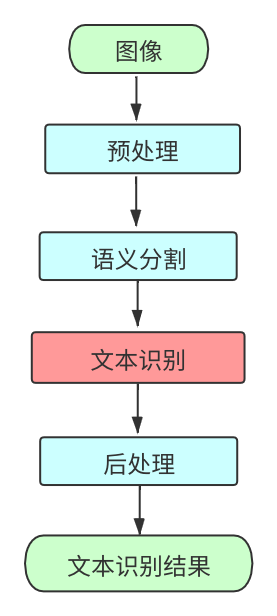
\includegraphics[width=0.8\textwidth]{OCR system.png}
			\end{center}
		\end{column}
	\end{columns}
\end{frame}

\begin{frame}[c]{}
	\begin{center}
		\begin{spacing}{2}
			{\large 面向\ALERT{语义分析}的\ALERT{文本识别}研究与实现!}
		\end{spacing}
		\includegraphics[width=.4\textwidth]{work.png}
	\end{center}
\end{frame}

\begin{frame}[c]{CRNN文本识别模型}{简要介绍}
\begin{columns}[t]
	\begin{column}[T]{5cm}
		CRNN\footnote{Shi B, \textit{el al}. An End-­to-­End Trainable Neural Network for Image Based Sequence Recognition and Its Application to Scene Text Recognition, \textbf{TPAMI}.} 思路:
		\begin{enumerate}
			\item CNN\footnote{本文使用的CRNN实现与原文略有不同:瓶颈层}:提取图像特征序列
			\item RNN:获取上下文信息
			\item CTC:变长序列映射 $\mathcal{B}: \mathbb{R}^{|L|} \rightarrow \mathbb{R}^{<|L|}$
		\end{enumerate}
	\end{column}
	\begin{column}[T]{6cm}
		\vspace{-2.5em}
		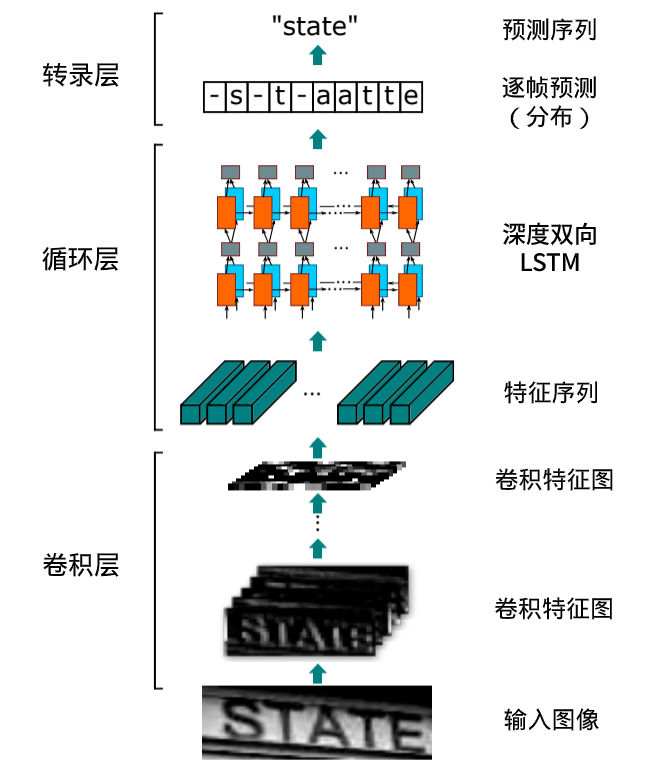
\includegraphics[width=.95\textwidth]{CRNN_arch.png}
	\end{column}
\end{columns}
\end{frame}

\begin{frame}[c]{基于语义分析的后处理}
	基于短语统计机器翻译(SMT)的方法\footnote{Chiu H w, \textit{el al}. Chinese Spelling Checker Based on Statistical
		Machine Translation. \textbf{ACL}.}:
	\begin{enumerate}
		\item 中文句子首先被分词,识别错误会导致一串\ALERT{单字}
		\item $n$-gram 检测成串单字是否为识别错误
		\item SMT 从候选结果中将错误翻译为正确形式
	\end{enumerate}

	\vspace{1.0em}
	
	基于 $n$-­gram 统计特征和迷惑集的方法\footnote{Huang Q, \textit{et al}. Chinese spelling check system based on tri­gram mode. \textbf{SIGHAN}.}:
	\begin{enumerate}
		\item 使用迷惑集枚举所有候选句子
		\item 使用动态规划找到 $n$-gram 分数最高的句子
		\item 使用 Laplace 平滑解决 $n$-gram 稀疏问题
	\end{enumerate}
\end{frame}

\begin{frame}[c]{本文贡献}
	\begin{enumerate}
		\item 构建了一个大规模合成数据集(160w)
		\item 研究并实现了基于 ConvS2S 字卷积的 OCR 后处理模块
		\item 研究并实现了基于 ALBERT 和 Transformer 的 OCR 后处理模块
		\item 与其他已有研究成果($n$-­gram+迷惑集)进行对比实验
	\end{enumerate}
\end{frame}

\section{基于字卷积的方法}

\begin{frame}[c]{ConvS2S 架构}
	\begin{columns}[t]
		\begin{column}[T]{5cm}
			{\footnotesize ConvS2S\footnote{Gehring J, \textit{et al}. Convolutional Sequence to Sequence Learning. \textbf{ICML}.} 为机器翻译模型,后在 NLPCC2018\footnote{{\fontsize{7}{7} \selectfont Ren H, \textit{el at}. A Sequence to Sequence Learning for Chinese Gram­matical Error Correction. \textbf{NLPCC}.}} 中用作中文语法修正}
			\begin{enumerate}
				\item {\footnotesize 输入和上文引入绝对值位置嵌入}
				\item {\footnotesize CNN激活单元:$\text{GLU}([A, B]) = A \otimes \sigma(B)$}
				\item {\footnotesize 编码器解码器架构:$p(y_{n+1}|y_1,\dots,y_n,\textbf{e})$}
				\item {\footnotesize 多步注意力:\\ 结合编码层和解码层的信息}
			\end{enumerate}
		\end{column}
		\begin{column}[T]{6cm}
			\vspace{-2.5em}
			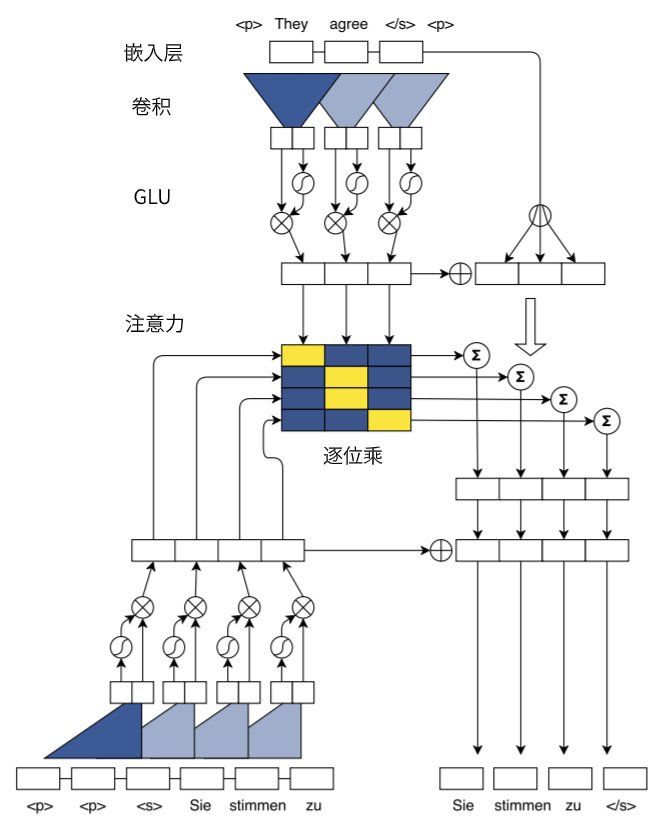
\includegraphics[width=.95\textwidth]{CS2S_arch.png}
		\end{column}
	\end{columns}
\end{frame}

\begin{frame}[c]{ConvS2S 架构}{多步注意力}
{\footnotesize
	带位置信息的嵌入表示:
	\begin{itemize}
		\item 输入 $E = (w_1 + p_1, \cdots, w_m + p_m) \in \mathbb{R}^{m \times f}$
		\item 上文内容 $G \in \mathbb{R}^{n \times f}$
	\end{itemize}

	对解码层第 $l$ 层,多步注意力结合卷积层输出 $\hat{H}_D^l$ 和编码层最终输出 $H^L_E$:
	\begin{align}
		Z_E^L &= \text{affine}_{h \rightarrow f}(H_E^L) \\
		C^l &= \text{Attention}(\text{affine}_{h \rightarrow f}(\hat{H}_D^l) + G, Z_E^L, Z_E^L + E) \in \mathbb{R}^{n \times f}\\
		H_D^l &= \hat{H}^l_D + C^l W_c
	\end{align}
	
	缩放点乘注意力:
	\begin{align}
		\text{Attention} (Q, K, V) &= \text{softmax}(\frac{QK^\top}{\sqrt{d_k}}) V \\
		\text{softmax}(X)_{ij} &= \frac{\exp(X_{ij})}{\sum_j \exp(X_{ij})}
	\end{align}
}%
\end{frame}

\section{基于语言模型和 Transformer 的方法}

\begin{frame}[c]{Transformer 机器翻译}{简要介绍}
	\begin{columns}[t]
		\begin{column}[T]{5cm}
			Transformer\footnote{Vaswani A, \textit{et al}. Attention is All you Need. \textbf{NIPS}.} 特点:
			\begin{enumerate}
				\item 编码器解码器架构
				\item 只使用\ALERT{自}注意力 $Q = K = V$
				\item 注意力中引入掩码
				\item 使用多头注意力学习更多特征
				\item 三角函数族位置编码
			\end{enumerate}
		\end{column}
		\begin{column}[T]{5cm}
			\vspace{-2.5em}
			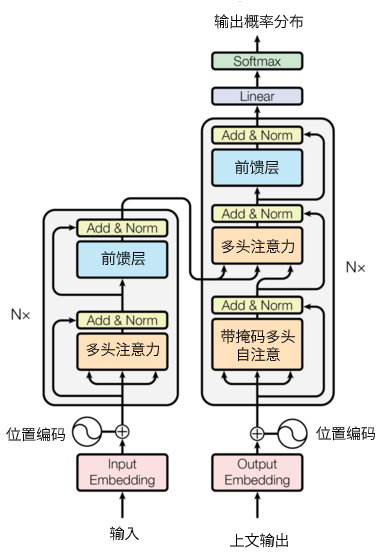
\includegraphics[width=.95\textwidth]{transformer.png}
		\end{column}
	\end{columns}
\end{frame}

\begin{frame}[c]{BERT 语言模型}{简要介绍}
	BERT\footnote{{\fontsize{7}{7} \selectfont Devlin J, \textit{et al}. Bert: Pre­training of deep bidirectional transformers for language understanding.}} 特点:
	\begin{enumerate}
		\item 类似 Transformer 编码层
		\item 两个无监督任务,适合大规模预训练:
		\begin{enumerate}
			\item \ALERT{带掩码的语言模型(Masked LM)}:预测被随机替换成\texttt{[MASK]}或\ALERT{随机词}的内容
			\item \Comment{下一句预测(NSP)}
		\end{enumerate}
		\item 预训练后轻松微调到各种下游任务
	\end{enumerate}

	ALBERT\footnote{{\fontsize{7}{7} \selectfont Lan Z, \textit{et al}. ALBERT: A Lite BERT for Self-­supervised Learning of Language Representations. \textbf{ICLR}.}}:
	\begin{enumerate}
		\item 所有层全部共享相同的参数,极大减小模型大小
		\item 使用句子顺序任务(SOP)替换掉 NSP 任务
	\end{enumerate}
\end{frame}

\begin{frame}[c]{基于 ALBERT\&Transformer 的方法}
	\only<1>{
		\begin{center}
			\begin{spacing}{2}
				{\large \ALERT{机器翻译模型 + 预训练语言模型?}}
			\end{spacing}
			\includegraphics[width=.5\textwidth]{MT_LM.png}
		\end{center}
	}%

	\only<2>{
		{\footnotesize
			\begin{columns}[t]
				\begin{column}[T]{5.5cm}
					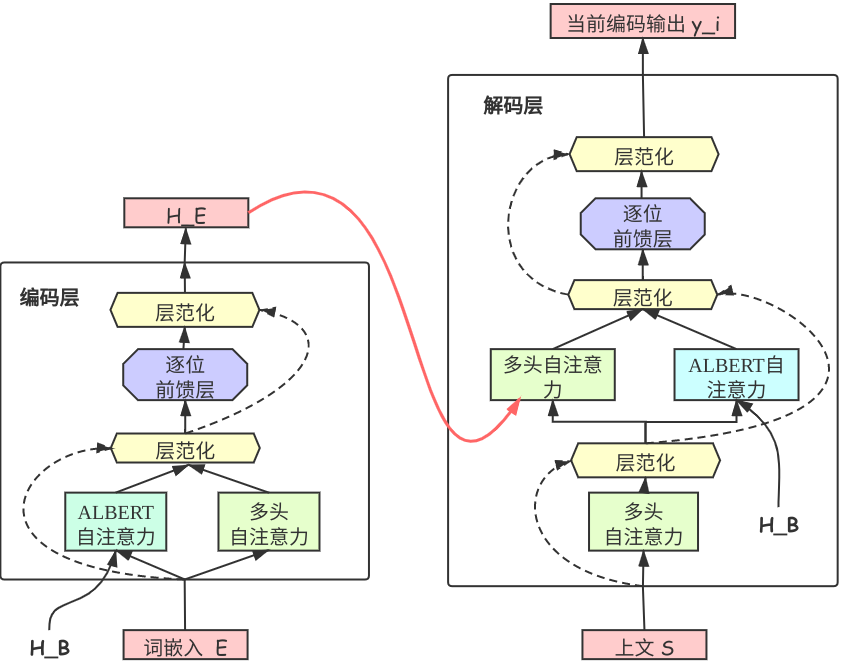
\includegraphics[width=1.1\textwidth]{ALBERT_NMT.png}
				\end{column}
				\begin{column}[T]{4cm}
					BERT-NMT\footnote{Zhu J, \textit{et al}. Incorporating BERT into Neural Machine Transla­tion. \textbf{ICLR}.} 机器翻译:
					\begin{enumerate}
						\item 在编码器解码器中引入 BERT 语言模型
						\item 使用 drop-net 正则化 BERT 带来的过拟合
					\end{enumerate} 
				\end{column}
			\end{columns}
		}%
	}
	
	\only<3>{
		{\footnotesize
		\begin{columns}[t]
			\begin{column}[T]{5cm}
				\ALERT{本文提出的改进:}
				\begin{enumerate}
					\item 将 BERT-NMT\footnote{Zhu J, \textit{et al}. Incorporating BERT into Neural Machine Transla­tion. \textbf{ICLR}.} 迁移为 OCR 语义修正后处理
					\item 将 BERT 替换为 ALBERT
					\item 取消分词
					\item 对输入和输出的嵌入层共享同一个词嵌入表
				\end{enumerate}
			\end{column}
			\begin{column}[T]{5cm}
				\hspace*{-2.5em}
				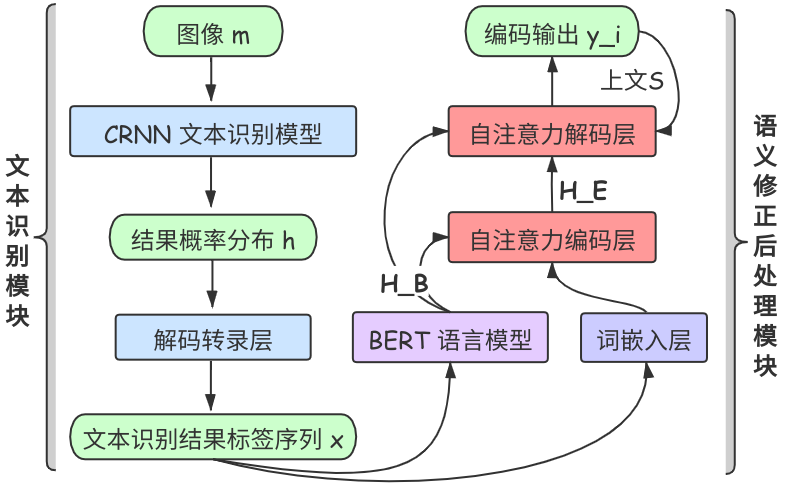
\includegraphics[width=1.3\textwidth]{overall.png}
			\end{column}
		\end{columns}
		}%
	}

\only<4>{
	{\footnotesize
		\begin{columns}[t]
			\begin{column}[T]{5cm}
				\ALERT{本文提出的改进:}
				\begin{enumerate}
					\item 将 BERT-NMT\footnote{Zhu J, \textit{et al}. Incorporating BERT into Neural Machine Transla­tion. \textbf{ICLR}.} 迁移为 OCR 识别语义修正后处理
					\item 将 BERT 替换为 ALBERT
					\item 取消分词
					\item 对输入和输出的嵌入层共享同一个 Lookup table
				\end{enumerate}
			\end{column}
			\begin{column}[T]{5cm}
				\hspace*{-2.5em}
				\includegraphics[width=1.3\textwidth]{overall_highlighted.png}
			\end{column}
		\end{columns}
	}%
}
\end{frame}

\section{实验验证}

\begin{frame}[c]{数据集和实验设计}
	\begin{columns}[t]
		{\scriptsize
		\begin{column}[T]{5cm}
			没有合适的开源数据集,所以自己合成 OCR 识别数据集:
			\begin{enumerate}
				\item 文本来源:THUCNews\footnote{Sum M, \textit{et al}. THUCTC: an efficient Chinese text classifier.} 新闻数据集
				\item 均匀选择 1,637,012 个文本行,长度固定 $18 \sim 20$
				\item 字典大小 $6425$
				\item 多种数据增强:70种不同字体,高斯噪声背景,随机文本畸变,色相抖动...
			\end{enumerate}
			
			\ALERT{构造语义修正后处理数据集:}
			\begin{enumerate}
				\item 按 $8:2$ 划分训练集和测试集(327,403)
				\item 使用 OCR 数据集训练 CRNN
				\item 使用训练得到的 CRNN 识别整个数据集构造识别结果与正确结果数据对
				\item 下采样正确识别的结果
			\end{enumerate}
		\end{column}
		}%
		\begin{column}[T]{5cm}
			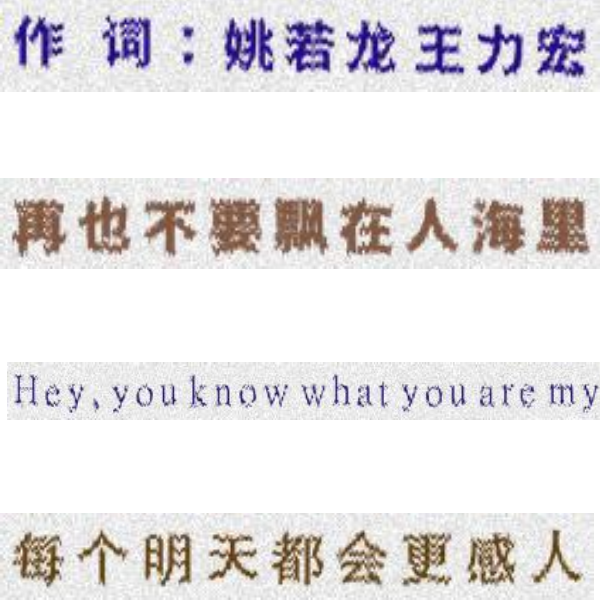
\includegraphics[width=\textwidth]{dataset_example.png}
		\end{column}
	\end{columns}
\end{frame}

\begin{frame}[c]{模型训练}
	\begin{enumerate}
		\item ConvS2S 训练收敛速度更快
		\item ConvS2S 过拟合了
		\item Transformer 训练更加平缓,没有过拟合
	\end{enumerate}
	\begin{columns}[t]
		\begin{column}[T]{5cm}
			\begin{figure}
				\centering
				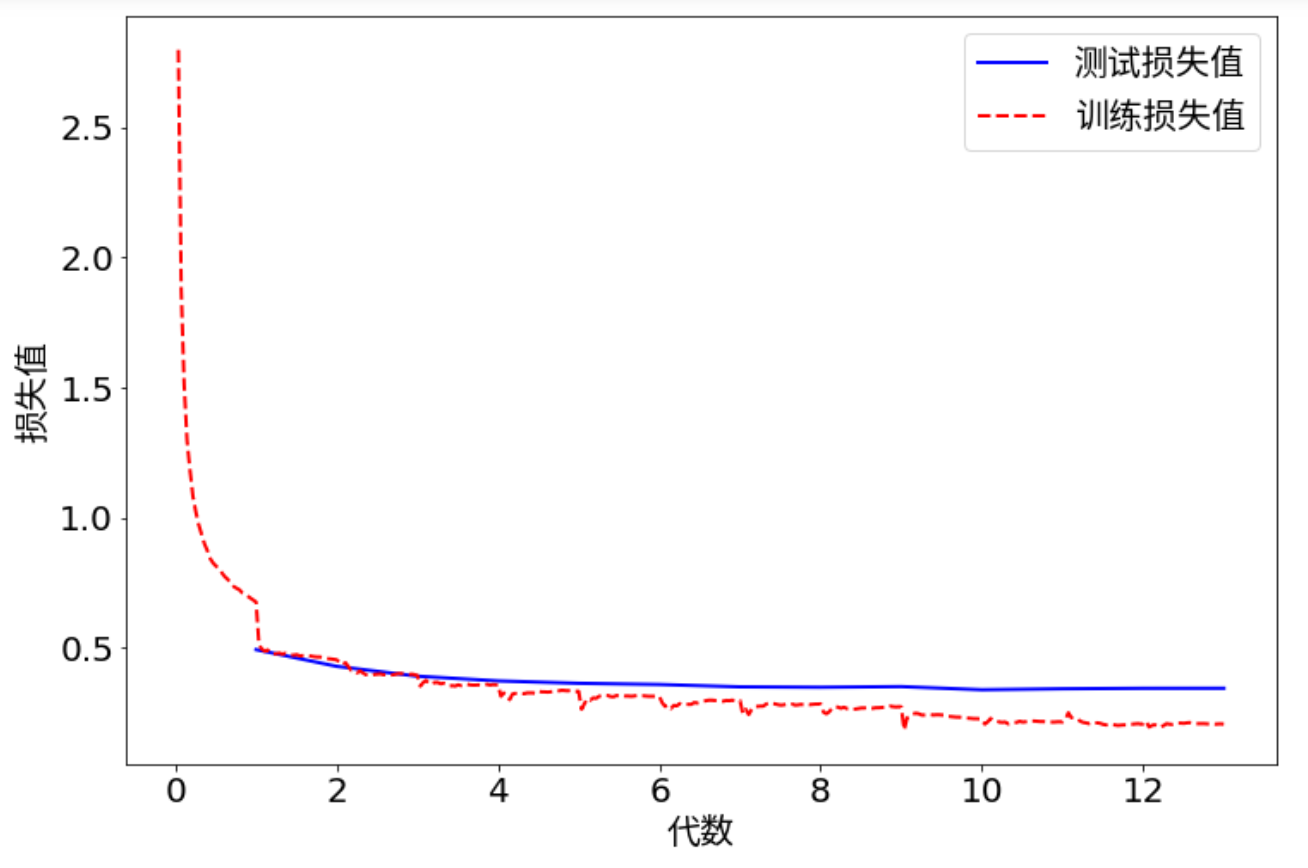
\includegraphics[width=\textwidth]{loss_cs2s.png}
				\caption{{\scriptsize ConvS2S 的训练曲线}}
			\end{figure}
		\end{column}
		\begin{column}[T]{5cm}
			\begin{figure}
				\centering
				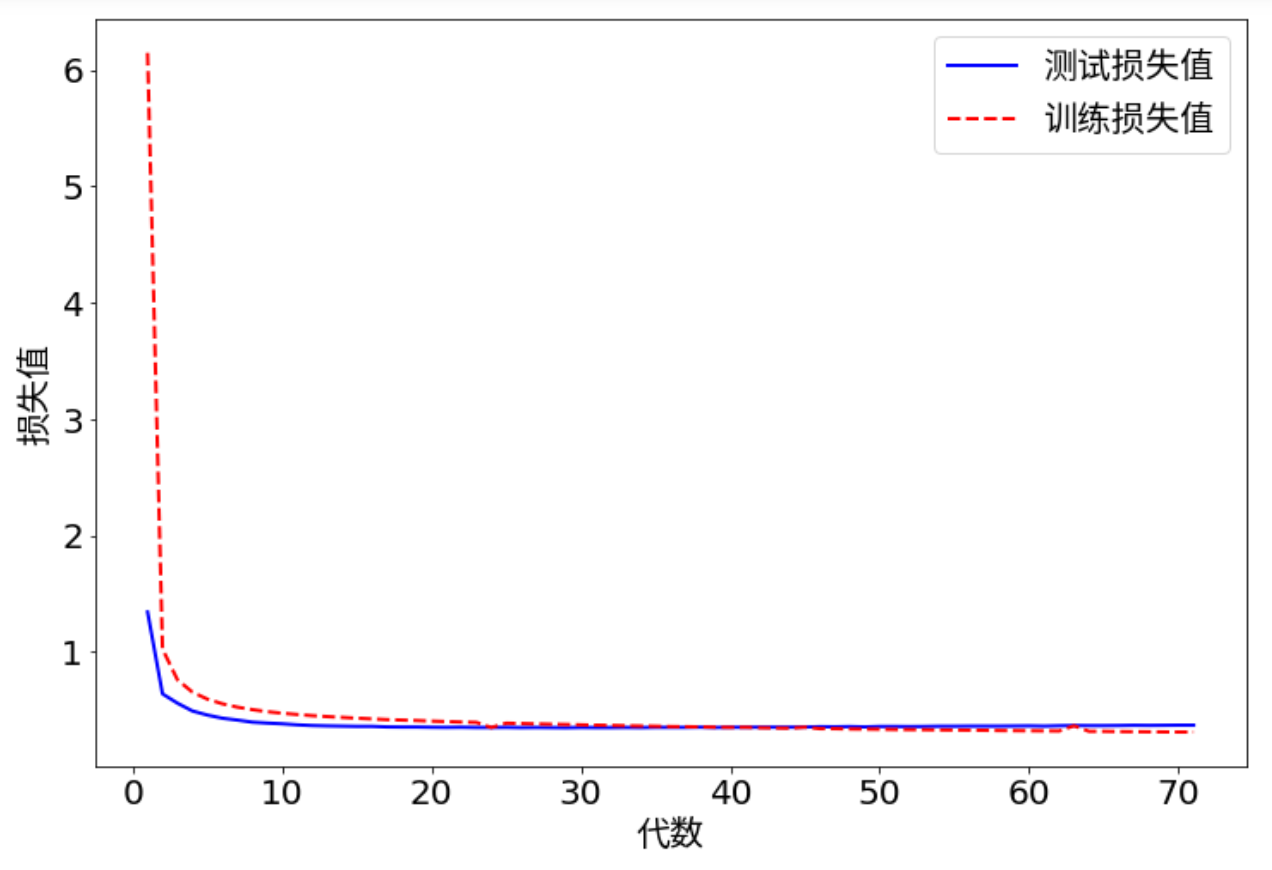
\includegraphics[width=\textwidth]{loss_transformer.png}
				\caption{{\scriptsize Transformer 的训练曲线}}
			\end{figure}
		\end{column}
	\end{columns}
\end{frame}

\begin{frame}[c]{实验结果}
	\vspace{-1.5em}
	\begin{columns}[t]
		\begin{column}[T]{.4\linewidth}
			{\scriptsize
			评价指标:
			\begin{enumerate}
				\item 完整匹配(EM)精确度
				\item Levenshtein 编辑距离归一化分数
			\end{enumerate}
			结论:
			\begin{enumerate}
				\item 基于 $n$-­gram 和迷惑集的传统方法效果不好
				\item ConvS2S 修正效果明显,略好于 Transformer
				\item ALBERT 对 Transformer 性能有帮助
				\item drop-net 率推荐使用 $0.4$
			\end{enumerate}
			}%
		\end{column}
		\begin{column}[T]{.55\linewidth}
			\begin{table}
				\scriptsize
				\caption[]{{\scriptsize drop-net 率参数调整实验结果}}
				\begin{tabular}{c c c}
					\hline
					drop-net 率 & EM 精确度 & Levenshtein 分数 \\
					\hline
					0.0 & 0.8320 & 94.3315 \\
					0.1 & 0.8347 & 94.2958 \\
					0.4 & \ALERT{0.8483} & \ALERT{94.3760} \\
					1.0 & 0.8453 & 94.3633 \\
					\hline
				\end{tabular}
			\end{table}
		\end{column}
	\end{columns}
\begin{table}
	\scriptsize
	\caption[]{{\scriptsize 对比实验结果}}
	\begin{tabular}{c c c}
		\hline
		方法名称 & EM 精确度 & Levenshtein 分数 \\
		\hline
		CRNN & 0.6420 & 94.0595 \\
		CRNN + $n$-gram & 0.6427 & 94.0927 \\
		CRNN + ConvS2S & 0.8461 & 94.3130 \\
		CRNN + Transformer & 0.8421 & 94.2802 \\
		CRNN + ALBERT-Transformer & \ALERT{0.8483} & \ALERT{94.3760} \\
		\hline
	\end{tabular}
\end{table}
\end{frame}

\begin{frame}[c]{实验结果分析}
\vspace{-2em}
\begin{table}
	\scriptsize
	\caption[]{{\scriptsize 基于语义分析的后处理修正模块成功案例}}
	\centering
	\begin{tabular}{c c}
		\hline
		OCR 识别结果 & 英格兰银行的通货膨\ALERT{服}目\ALERT{模}为2\%。根据国 \\
		识别错误类型 & 替换+插入 \\
		语义修正结果 & 英格兰银行的通货膨\ALERT{胀}目\ALERT{标}为2\%。根据国\ALERT{际} \\
		\hline
		& \\
		\hline
		OCR 识别结果 & 仍由民政部与\ALERT{罔}家\ALERT{休}体育\ALERT{鹅}局具休制定和\ALERT{宵}施。 \\
		识别错误类型 & 删除+替换 \\
		语义修正结果 & 仍由民政部与\ALERT{国}家体育总局具体制定和实施 \\
		\hline
	\end{tabular}
\end{table}

\begin{table}
	\scriptsize
	\caption[]{{\scriptsize 基于语义分析的后处理修正模块失败案例}}
	\centering
	\begin{tabular}{c c}
		\hline
		OCR 识别结果 & 活家禽批发商会预计,零\ALERT{傅}价约为每斤2\ALERT{G}6元 \\
		语义修正结果(ALBERT-Transformer) & 活家禽批发商会预计,零售价约为每斤66元 \\
		语义修正结果(ConvS2S) & 活家禽批发商会预计,零售约为每斤2G6元 \\
		实际正确结果 & 活家禽批发商会预计,零售价约为每斤26元 \\
		\hline
		& \\
		\hline
		OCR 识别结果 & “我\ALERT{冈图}密室部分,\ALERT{区}(指\ALERT{因}佩慈)\ALERT{因因}不可 \\
		语义修正结果(ALBERT-Transformer) & “我们紧密室部分,谢(指导佩慈)发现不可 \\
		语义修正结果(ConvS2S) & “我们亲密室部分,谢(指纹佩慈)因为不可 \\
		实际正确结果 & “我负责密室部分,她(指吴佩慈)负责不可 \\
		\hline
	\end{tabular}
\end{table}
\end{frame}

\begin{frame}[c]{实验结果分析}
	\vspace{-2em}
	\begin{table}
		\scriptsize
		\caption[]{{\scriptsize 基于语义分析的后处理修正模块成功案例}}
		\centering
		\begin{tabular}{c c}
			\hline
			OCR 识别结果 & 中国外\ALERT{论}交\ALERT{马}中\ALERT{.}心公布,人民币\ALERT{见}美元9日 \\
			识别错误类型 & 删除+替换 \\
			语义修正结果 & 中国外\ALERT{汇}交\ALERT{易}中心公布,人民币\ALERT{兑}美元9日中 \\
			\hline
			& \\
			\hline
			OCR 识别结果 &\ALERT{达}一点当\ALERT{燃丹}益于饰\ALERT{梅}者金范的端\ALERT{止}外形, \\
			识别错误类型 & 替换 \\
			语义修正结果 & \ALERT{这}一点当\ALERT{然得}益于饰\ALERT{掩}者金范的端\ALERT{正}外形,不 \\
			\hline
		\end{tabular}
	\end{table}
	
	\begin{table}
		\scriptsize
		\caption[]{{\scriptsize 基于语义分析的后处理修正模块失败案例}}
		\centering
		\begin{tabular}{c c}
			\hline
			OCR 识别结果 & 更不知道到底欠了多少线,不\ALERT{遇退}他知道一\ALERT{黏}, \\
			语义修正结果(ALBERT-Transformer) & 更不知道到底欠了多少钱,不过\ALERT{过}他知道一点 \\
			语义修正结果(ConvS2S) & 更不知道到底欠了多少钱,不过他知道一点 \\
			实际正确结果 & 更不知道到底欠了多少钱,不过他知道一点 \\
			\hline
			& \\
			\hline
			OCR 识别结果 & 王尽士念丽一闹门匿锯很风等 \\
			语义修正结果(ALBERT-Transformer) & 王女士表示,一家人\ALERT{数据等风险。他认为只要} \\
			语义修正结果(ConvS2S) & 王女士表示,\ALERT{在}一家人\ALERT{透露,据很风险,只要} \\
			实际正确结果 & 王女士表示,这一家人的遭遇很让人感触, \\
			\hline
		\end{tabular}
	\end{table}
\end{frame}

\section{总结与展望}

\begin{frame}[c]{总结与展望}
	总结:
	\begin{enumerate}
		\item OCR 语义修正可以视为一种特殊的机器翻译
		\item 基于海量文本的预训练语言模型可以提供有效的语义信息
		\item 近距离局部信息可能更加重要(ConvS2S)
	\end{enumerate}
	展望:
	\begin{enumerate}
		\item 将文本识别模型的中间特征加入语义修正模型
		\item 更好的融合语言模型的特征
		\item 优化基于 ALBERT 和 Transformer 的方法的训练速度
	\end{enumerate}
\end{frame}

\begin{frame}[c]{}
	\begin{center}
		\begin{spacing}{2}
			{\LARGE \ALERT{欢迎各位老师点评指导} \\ \ALERT{谢谢观看!}}
		\end{spacing}
	\end{center}
\end{frame}

% \begin{frame}{test}
% 	Main text still in Gill Sans
% 	$$\frac{f}{f^4}$$
%
% 	But math is now different
% 	\Large
% 	$$\frac{f^2}{f^4}$$
% \end{frame}


\end{document}

